\chapter{5 Station Analysis L2 Variables \label{app:5savariables}}

This is a limited collection of analysis variables calculated as a part of the analysis presented in Chapter~\ref{chap:5sa_cleaning} and Chapter~\ref{chap:5sa_analysis}. 
Full definitions of each variable may be found in AraProc source code.

\section{\texttt{avg\_rms} \label{sec:rms}}

  The average root-mean-square ($RMS$, also referred to as $\sigma$) of noise portions of waveforms is calculated using a jackknife technique. 
  The full waveform is split into 50 segments and the RMS of the waveform without each segment is calculated in the so-called $RMS_{\text{all-but}}$. 
  Segments that contain non-thermal signals have an $RMS_{\text{all-but}}$ that is significantly less than the average of $RMS_{\text{all-but}}$ values for all segments. 
  Segments with an $RMS_{\text{all-but}}$ value more than one standard deviation lower than the mean of all other $RMS_{\text{all-but}}$ values are isolated. 
  Once all segments with non-thermal contributions are isolated, the $RMS$ is calculated over all remaining segments. 

  \begin{figure}
    \centering
    \begin{subfigure}[t]{0.48\textwidth}
      \centering
      \includegraphics[width=\textwidth]{sections/5sa-cleaning/images_variables/a2nu_1d_avg_rms_v.pdf}
    \end{subfigure}
    ~
    \begin{subfigure}[t]{0.48\textwidth}
      \centering
      \includegraphics[width=\textwidth]{sections/5sa-cleaning/images_variables/a2_10pct_1d_avg_rms_v.pdf}
    \end{subfigure}
    ~
    \begin{subfigure}[t]{0.48\textwidth}
      \centering
      \includegraphics[width=\textwidth]{sections/5sa-cleaning/images_variables/a2nu_2d_avg_rms_v_vs_avg_snr_v_rf.pdf}
    \end{subfigure}
    ~
    \begin{subfigure}[t]{0.48\textwidth}
      \centering
      \includegraphics[width=\textwidth]{sections/5sa-cleaning/images_variables/a2nu_2d_avg_rms_v_vs_global_max_corr_rf.pdf}
    \end{subfigure}
    \caption{
      Top, 1-dimensional distributions of simulated neutrinos following an $E^{-2}$ spectrum (top left) and data (top right) for the analysis variable \texttt{avg\_rms\_v}. 
      The distribution of data has had all cuts applied to RF events except for the final thermal LDA cut described in Section~\ref{sec:lda}.
      The purple curve (which exactly overlays the orange curve) shows these RF events, blue shows software triggered events, and green shows calibration pulser events.
      Bottom, 2-dimensional distributions of simulated neutrinos for the analysis variable \texttt{avg\_rms\_v} as a function of \texttt{avg\_snr\_v} and \texttt{global\_max\_corr\_v}.
    }
    \label{fig:avg_rms}
  \end{figure}

\pagebreak
\section{\texttt{avg\_rpr} and \texttt{csw\_rpr}}

    The root power ratio ($RPR$) approximates the maximum power in a waveform and divides it by the voltage of the noise background, in a calculation similar to the signal-to-noise ratio ($SNR$).
    The $RPR$ is calculated two ways, first by squaring the raw waveform, squaring each value (as the proxy for power), smoothing the squared waveform, and extracting the maximum value then dividing it by the $RMS$ of the noise background in the waveform via the calculation defined in Section~\ref{sec:rms}.
    The second method follows the same approach but uses the Coherently Summed Waveform instead of the raw waveform to perform the calculation.
    For both methods, the average $RPR$ is calculated over all like-polarization channels and returned.
    Example distributions are shown in Figure~\ref{fig:avg_rpr}.
  
    \begin{figure}
      \centering
      \begin{subfigure}[t]{0.48\textwidth}
        \centering
        \includegraphics[width=\textwidth]{sections/5sa-cleaning/images_variables/a2nu_1d_avg_rpr_v.pdf}
      \end{subfigure}
      ~
      \begin{subfigure}[t]{0.48\textwidth}
        \centering
        \includegraphics[width=\textwidth]{sections/5sa-cleaning/images_variables/a2_10pct_1d_avg_rpr_v.pdf}
      \end{subfigure}
      ~
      \begin{subfigure}[t]{0.48\textwidth}
        \centering
        \includegraphics[width=\textwidth]{sections/5sa-cleaning/images_variables/a2nu_2d_avg_rpr_v_vs_avg_snr_v_rf.pdf}
      \end{subfigure}
      ~
      \begin{subfigure}[t]{0.48\textwidth}
        \centering
        \includegraphics[width=\textwidth]{sections/5sa-cleaning/images_variables/a2nu_2d_avg_rpr_v_vs_global_max_corr_rf.pdf}
      \end{subfigure}
      \caption{
        Top, 1-dimensional distributions of simulated neutrinos following an $E^{-2}$ spectrum (top left) and data (top right) for the analysis variable \texttt{avg\_rpr\_v}. 
        The distribution of data has had all cuts applied to RF events except for the final thermal LDA cut described in Section~\ref{sec:lda}.
        The purple curve (which exactly overlays the orange curve) shows these RF events, blue shows software triggered events, and green shows calibration pulser events.
        Bottom, 2-dimensional distributions of simulated neutrinos for the analysis variable \texttt{avg\_rpr\_v} as a function of \texttt{avg\_snr\_v} and \texttt{global\_max\_corr\_v}.
      }
      \label{fig:avg_rpr}
    \end{figure}

\pagebreak
\section{\texttt{avg\_s2}}

  \texttt{avg\_s2} is a measure of signal causality constructed similarly to the \texttt{wavefront\_rms}. 
  For all antennas of like-polarization, the time of maximum peak-to-peak voltage in any 20 nanosecond window of every waveform is identified. 
  Again assuming that a plane wave arrived at each antenna at the determined time of maximal voltage separation, for each pair of antennas we calculate the average spacetime interval as
  \begin{equation}
    s^2 = \Delta r^2 - ({c}{n})^2 \Delta t^2
    \label{eq:avg_s2}
  \end{equation}
  where $\Delta r$ is the distance between a pair of antennas, $c$ is the speed of light in a vacuum, $n$ is the index of refraction of the medium, and  $\Delta t$ is the time difference between the assumed signal arrival in each antenna (the time of maximal voltage separation).
  When $s^2$ is positive this indicates a causal relationship between signals in each channel. 
  When $s^2$ is negative, this indicates an acausal, non-physical signal that would not be expected of an arriving impulsive signal.
  We take the average $s^2$ calculated over all antenna pairs of like-polarization and report this as the \texttt{avg\_s2}.
  Example distributions are shown in Figure~\ref{fig:avg_s2}.

  \begin{figure}
    \centering
    \begin{subfigure}[t]{0.48\textwidth}
      \centering
      \includegraphics[width=\textwidth]{sections/5sa-cleaning/images_variables/a2nu_1d_avg_s2_v.pdf}
    \end{subfigure}
    ~
    \begin{subfigure}[t]{0.48\textwidth}
      \centering
      \includegraphics[width=\textwidth]{sections/5sa-cleaning/images_variables/a2_10pct_1d_avg_s2_v.pdf}
    \end{subfigure}
    ~
    \begin{subfigure}[t]{0.48\textwidth}
      \centering
      \includegraphics[width=\textwidth]{sections/5sa-cleaning/images_variables/a2nu_2d_avg_s2_v_vs_avg_snr_v_rf.pdf}
    \end{subfigure}
    ~
    \begin{subfigure}[t]{0.48\textwidth}
      \centering
      \includegraphics[width=\textwidth]{sections/5sa-cleaning/images_variables/a2nu_2d_avg_s2_v_vs_global_max_corr_rf.pdf}
    \end{subfigure}
    \caption{
      Top, 1-dimensional distributions of simulated neutrinos following an $E^{-2}$ spectrum (top left) and data (top right) for the analysis variable \texttt{avg\_s2\_v}. 
      The distribution of data has had all cuts applied to RF events except for the final thermal LDA cut described in Section~\ref{sec:lda}.
      The purple curve (which exactly overlays the orange curve) shows these RF events, blue shows software triggered events, and green shows calibration pulser events.
      Bottom, 2-dimensional distributions of simulated neutrinos for the analysis variable \texttt{avg\_s2\_v} as a function of \texttt{avg\_snr\_v} and \texttt{global\_max\_corr\_v}.
    }
    \label{fig:avg_s2}
  \end{figure}

\pagebreak
\section{\texttt{avg\_snr}}
  
    The average signal-to-noise ratio ($SNR$) is calculated using Equation~\ref{eq:snr} by identifying the maximum peak-to-peak voltage ($V_{\text{max}} - V_{\text{min}}$) within an 20~ns window, dividing this value by two (to quantify the amount of ``signal'' in the waveform), then dividing this number by the $RMS$ voltage for the waveform as defined in Section~\ref{sec:rms} (to quantify the ``noise'', also referred to as $\sigma$).
    The $SNR$ values in each like-polarization channel are averaged together to achieve the average $SNR$.
    Example distributions are shown in Figure~\ref{fig:avg_snr}.
  
    \begin{figure}
      \centering
      \begin{subfigure}[t]{0.48\textwidth}
        \centering
        \includegraphics[width=\textwidth]{sections/5sa-cleaning/images_variables/a2nu_1d_avg_snr_v.pdf}
      \end{subfigure}
      ~
      \begin{subfigure}[t]{0.48\textwidth}
        \centering
        \includegraphics[width=\textwidth]{sections/5sa-cleaning/images_variables/a2_10pct_1d_avg_snr_v.pdf}
      \end{subfigure}
      ~
      \begin{subfigure}[t]{0.48\textwidth}
        \centering
        \includegraphics[width=\textwidth]{sections/5sa-cleaning/images_variables/a2nu_2d_global_max_corr_vs_avg_snr_v_rf.pdf}
      \end{subfigure}
      \caption{
        Top, 1-dimensional distributions of simulated neutrinos following an $E^{-2}$ spectrum (top left) and data (top right) for the analysis variable \texttt{avg\_snr\_v}. 
        The distribution of data has had all cuts applied to RF events except for the final thermal LDA cut described in Section~\ref{sec:lda}.
        The purple curve (which exactly overlays the orange curve) shows these RF events, blue shows software triggered events, and green shows calibration pulser events.
        Bottom, 2-dimensional distributions of simulated neutrinos for the analysis variable \texttt{avg\_snr\_v} as a function of \texttt{global\_max\_corr\_v}.
      }
      \label{fig:avg_snr}
    \end{figure}
  
\section{\texttt{corr\_snr}}

  The correlation $SNR$ is calculated by identifying all pairs of like-polarization channels, calculating the cross correlation function of their two waveforms, then determining the SNR (following Equation~\ref{eq:snr}) of the cross correlation function for each pair. 
  The average over the SNR for each pair's correlation function is what is returned as the \texttt{corr\_snr}.
  Example distributions are shown in Figure~\ref{fig:corr_snr}.
  
  \begin{figure}
    \centering
    \begin{subfigure}[t]{0.48\textwidth}
      \centering
      \includegraphics[width=\textwidth]{sections/5sa-cleaning/images_variables/a2nu_1d_corr_snr_v.pdf}
    \end{subfigure}
    ~
    \begin{subfigure}[t]{0.48\textwidth}
      \centering
      \includegraphics[width=\textwidth]{sections/5sa-cleaning/images_variables/a2_10pct_1d_corr_snr_v.pdf}
    \end{subfigure}
    ~
    \begin{subfigure}[t]{0.48\textwidth}
      \centering
      \includegraphics[width=\textwidth]{sections/5sa-cleaning/images_variables/a2nu_2d_corr_snr_v_vs_avg_snr_v_rf.pdf}
    \end{subfigure}
    ~
    \begin{subfigure}[t]{0.48\textwidth}
      \centering
      \includegraphics[width=\textwidth]{sections/5sa-cleaning/images_variables/a2nu_2d_corr_snr_v_vs_global_max_corr_rf.pdf}
    \end{subfigure}
    \caption{
      Top, 1-dimensional distributions of simulated neutrinos following an $E^{-2}$ spectrum (top left) and data (top right) for the analysis variable \texttt{corr\_snr\_v}. 
      The distribution of data has had all cuts applied to RF events except for the final thermal LDA cut described in Section~\ref{sec:lda}.
      The purple curve (which exactly overlays the orange curve) shows these RF events, blue shows software triggered events, and green shows calibration pulser events.
      Bottom, 2-dimensional distributions of simulated neutrinos for the analysis variable \texttt{corr\_snr\_v} as a function of \texttt{avg\_snr\_v} and \texttt{global\_max\_corr\_v}.
    }
    \label{fig:corr_snr}
  \end{figure}
  
\pagebreak
\section{\texttt{csw\_snr} \label{sec:csw}}
  
    \begin{figure}[!ht]
      \centering
      \centering
      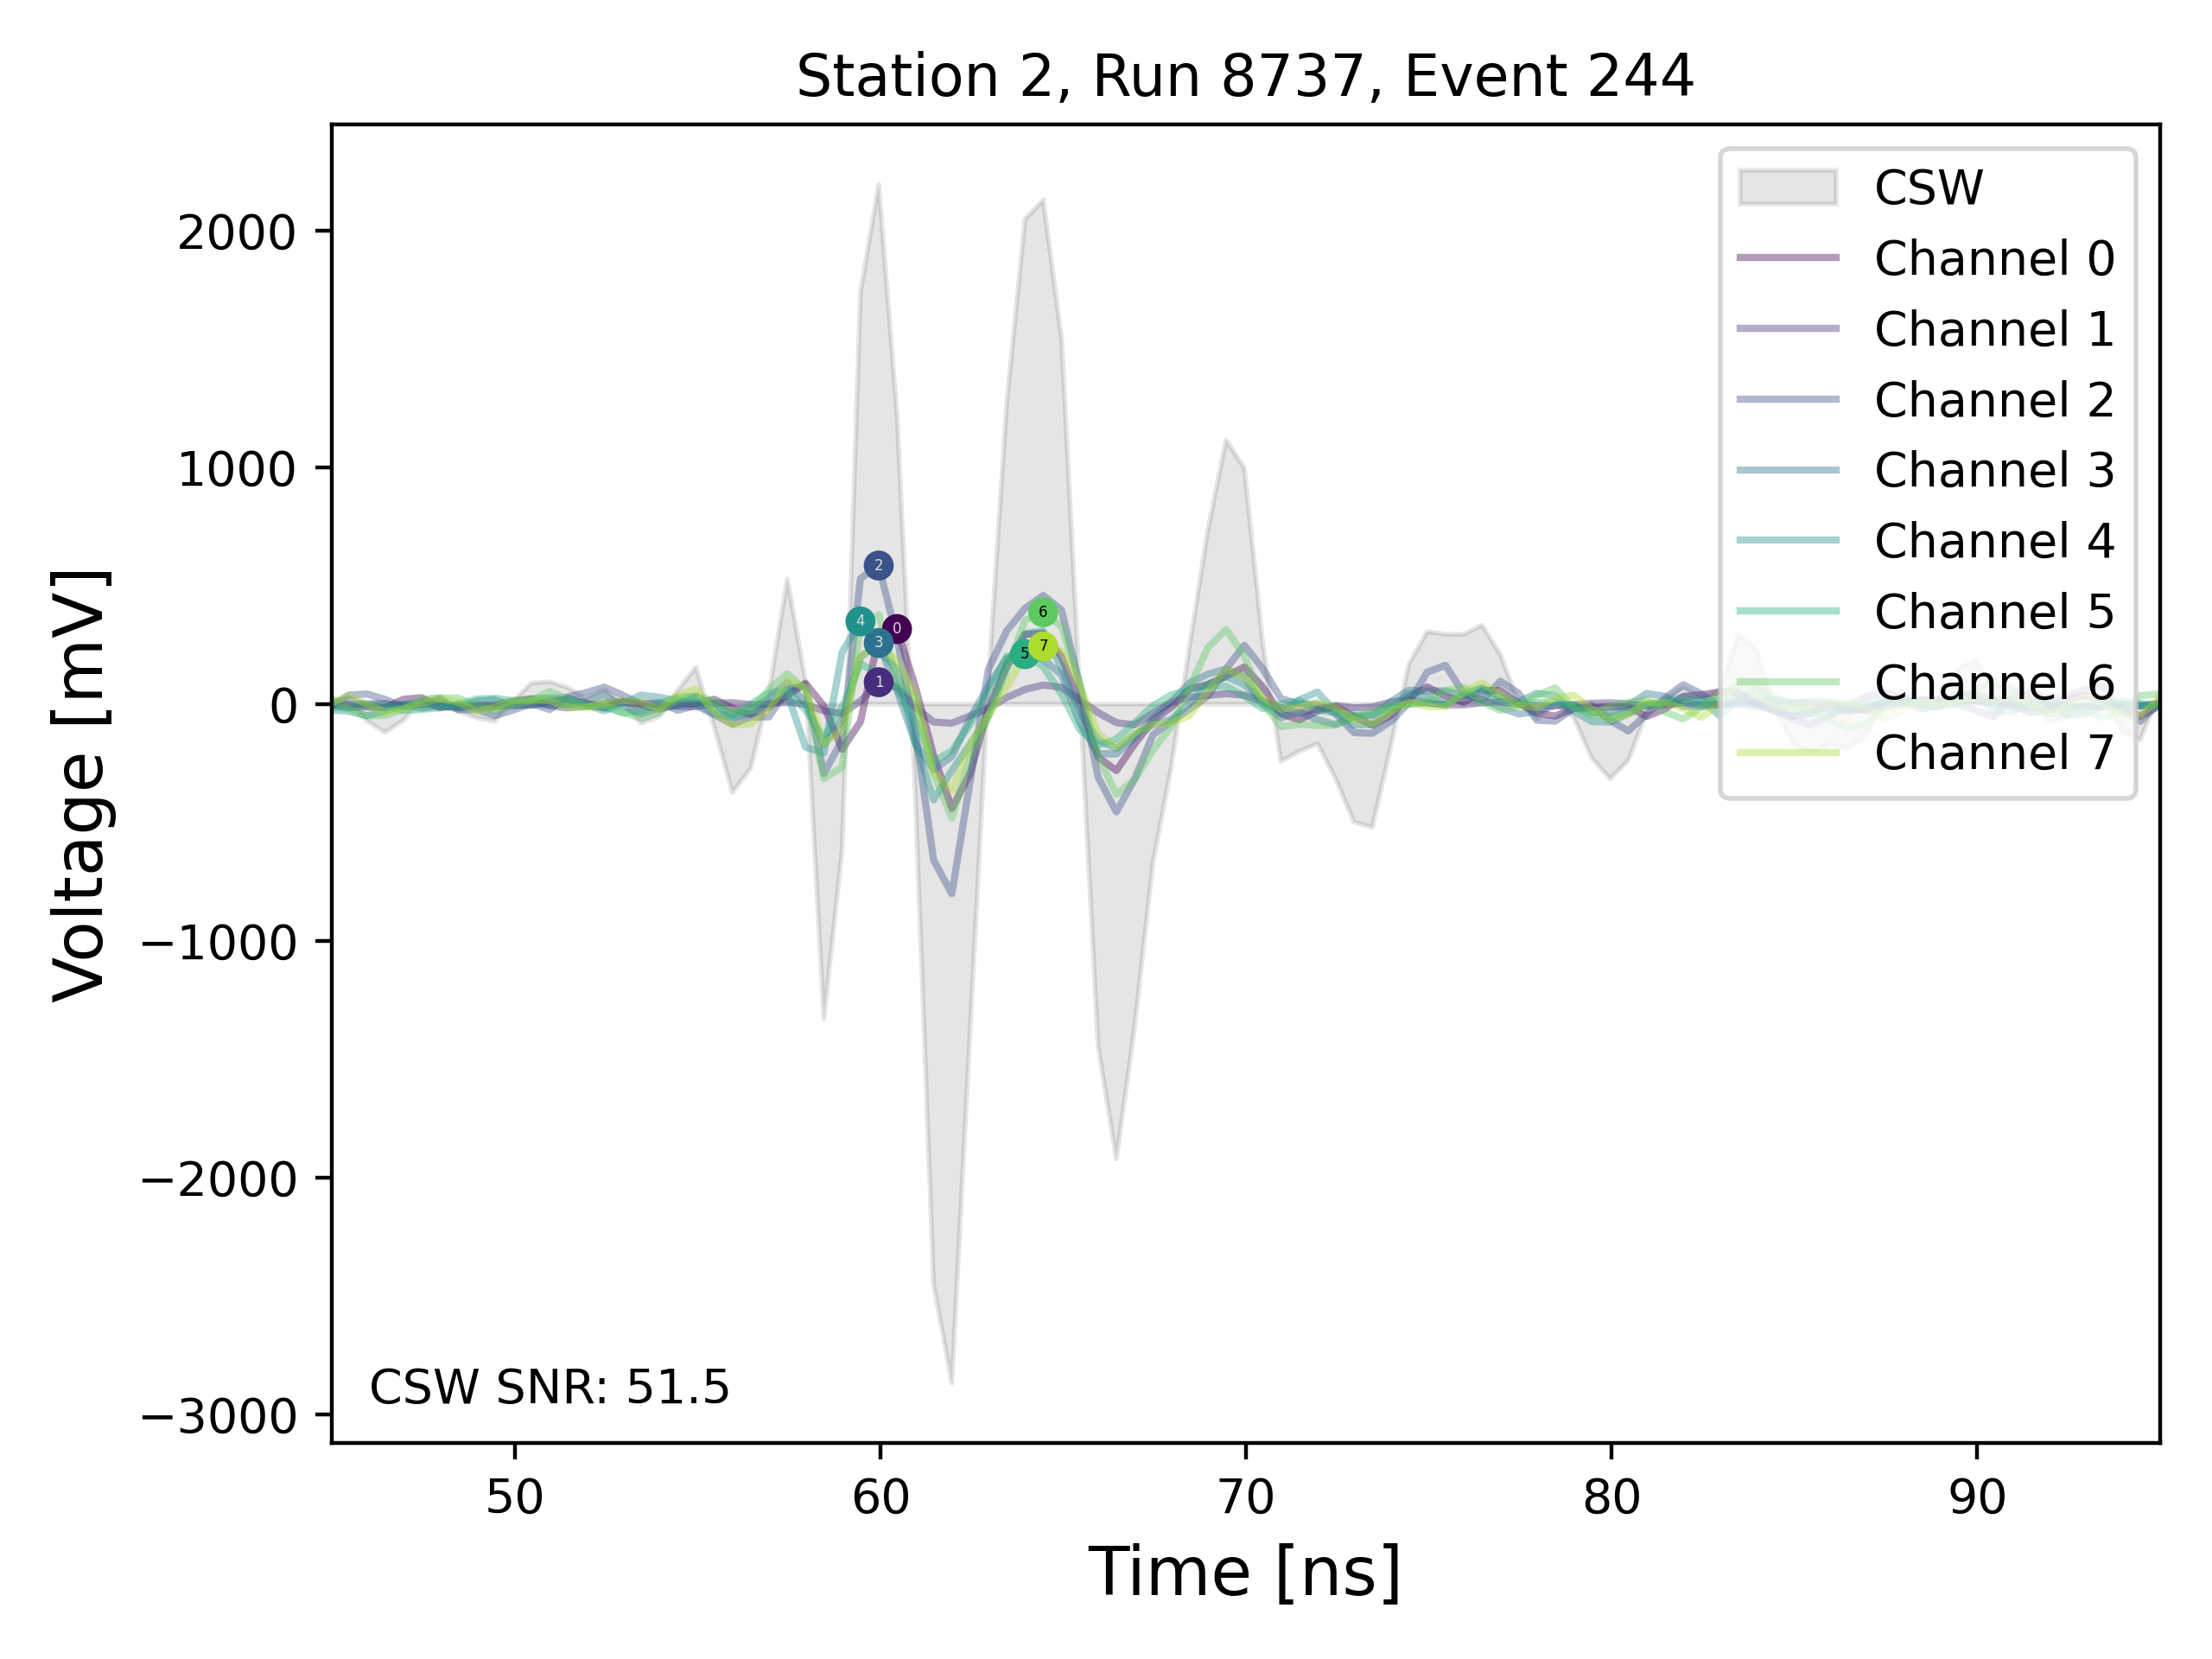
\includegraphics[width=0.75\textwidth]{sections/5sa-cleaning/images_variables/csw_s2_r8737_e244.png}
      \caption{
        Example of a Coherently Summed Waveform (CSW, grey) and the waveforms composing the CSW. 
        The circles on each channel mark the location of each waveform's maximum voltage.
      }
      \label{fig:csw}
    \end{figure}

    The Coherently Summed Waveform (CSW) SNR is calculated by determining the SNR of the CSW composed of all like-polarization antennas. 
    The CSW is constructed first by reconstructing an events arrival direction using the interferometric reconstruction algorithm described in Section~\ref{sec:reco}. 
    The expected arrival time of signals from this reconstructed location to each like-polarization antenna are used to translate each waveform in time. 
    For highly correlated signals, the peak of each waveform should now align at the same time bin. 
    When each waveform is added together, the signal increases roughly at a factor of $N_a$ (the number of antennas) but the noise increases at a factor of roughly $\sqrt{N_a}$. 
    This allows highly correlated signals that are low in signal strength to rise out of the noise floor, increasing their chance of passing all analysis cuts. 
    Before summing all waveforms, each waveform's time delay is allowed to change by up to 20~ns to maximize the CSW.
    An example of a CSW is shown in Figure~\ref{fig:csw} and example distributions are shown in Figure~\ref{fig:csw_snr}.
  
    \begin{figure}
      \centering
      \begin{subfigure}[t]{0.48\textwidth}
        \centering
        \includegraphics[width=\textwidth]{sections/5sa-cleaning/images_variables/a2nu_1d_csw_snr_v.pdf}
      \end{subfigure}
      ~
      \begin{subfigure}[t]{0.48\textwidth}
        \centering
        \includegraphics[width=\textwidth]{sections/5sa-cleaning/images_variables/a2_10pct_1d_csw_snr_v.pdf}
      \end{subfigure}
      ~
      \begin{subfigure}[t]{0.48\textwidth}
        \centering
        \includegraphics[width=\textwidth]{sections/5sa-cleaning/images_variables/a2nu_2d_csw_snr_v_vs_avg_snr_v_rf.pdf}
      \end{subfigure}
      ~
      \begin{subfigure}[t]{0.48\textwidth}
        \centering
        \includegraphics[width=\textwidth]{sections/5sa-cleaning/images_variables/a2nu_2d_csw_snr_v_vs_global_max_corr_rf.pdf}
      \end{subfigure}
      \caption{
        Top, 1-dimensional distributions of simulated neutrinos following an $E^{-2}$ spectrum (top left) and data (top right) for the analysis variable \texttt{csw\_snr\_v}. 
        The distribution of data has had all cuts applied to RF events except for the final thermal LDA cut described in Section~\ref{sec:lda}.
        The purple curve (which exactly overlays the orange curve) shows these RF events, blue shows software triggered events, and green shows calibration pulser events.
        Bottom, 2-dimensional distributions of simulated neutrinos for the analysis variable \texttt{csw\_snr\_v} as a function of \texttt{avg\_snr\_v} and \texttt{global\_max\_corr\_v}.
      }
      \label{fig:csw_snr}
    \end{figure}

\pagebreak
\section{\texttt{global\_max\_corr} and \texttt{reco\_result\_*\_corr}}
  
  The cross correlation of all pairs of like-polarized antennas is performed on a sphere with a radius equal to the pulser's distance from the station's center (this is also called the ``nearby" reconstruction) and a sphere with a radius of 300 meters (called the ``distant" reconstruction). 
  %The reconstructed correlation is computed by determining which point on the sphere the signals must have come from to be maximally correlated.
  %The correlation is first computed between pairs of antennas where waveforms have been shifted in time according to the arrival delay of signals if they were to arrive from a certain location on the sphere. 
  %Once time-shifted, the two waveforms are cross correlated to obtain their correlation value. 
  %% What is the correlation? The maximum of the correlation function or the area under the curve or what? 
  %% Is the total correlation an average of the correlation between all antennas? 
  %It is a process that requires significant computation time as multiple locations on the sphere are tested in search of the best position on the sphere. 
  
  The maximum correlation in all four reconstructions (two polarizations, two distances) is saved to a variable called \texttt{global\_max\_corr} while the maximum correlation in horizontally and vertically polarized antennas separately are saved as \texttt{global\_max\_corr\_h} and \texttt{global\_max\_corr\_v}, respectively. Shown in Figure~\ref{fig:global_max_correlation} are example distributions of the \texttt{global\_max\_corr} variable.
  
    \begin{figure}
      \centering
      \begin{subfigure}[t]{0.48\textwidth}
        \centering
        \includegraphics[width=\textwidth]{sections/5sa-cleaning/images_variables/a2nu_1d_global_max_corr.pdf}
      \end{subfigure}
      ~
      \begin{subfigure}[t]{0.48\textwidth}
        \centering
        \includegraphics[width=\textwidth]{sections/5sa-cleaning/images_variables/a2_10pct_1d_global_max_corr.pdf}
      \end{subfigure}
      ~
      \begin{subfigure}[t]{0.48\textwidth}
        \centering
        \includegraphics[width=\textwidth]{sections/5sa-cleaning/images_variables/a2nu_2d_global_max_corr_vs_avg_snr_v_rf.pdf}
      \end{subfigure}
      \caption{
        Top, 1-dimensional distributions of simulated neutrinos following an $E^{-2}$ spectrum (top left) and data (top right) for the analysis variable \texttt{global\_max\_corr}. 
        The distribution of data has had all cuts applied to RF events except for the final thermal LDA cut described in Section~\ref{sec:lda}.
        The purple curve (which exactly overlays the orange curve) shows these RF events, blue shows software triggered events, and green shows calibration pulser events.
        Bottom, 2-dimensional distributions of simulated neutrinos for the analysis variable \texttt{global\_max\_corr} as a function of \texttt{avg\_snr\_v}.
      }
      \label{fig:global_max_correlation}
    \end{figure}

\section{\texttt{hilbert\_snr}}

    The Hillbert SNR is the average SNR of each waveform from like-polarized antennas after being Hilbert Enveloped. 
    Example distributions are show in in Figure~\ref{fig:hilbert_snr}.
  
    \begin{figure}
      \centering
      \begin{subfigure}[t]{0.48\textwidth}
        \centering
        \includegraphics[width=\textwidth]{sections/5sa-cleaning/images_variables/a2nu_1d_hilbert_snr_v.pdf}
      \end{subfigure}
      ~
      \begin{subfigure}[t]{0.48\textwidth}
        \centering
        \includegraphics[width=\textwidth]{sections/5sa-cleaning/images_variables/a2_10pct_1d_hilbert_snr_v.pdf}
      \end{subfigure}
      ~
      \begin{subfigure}[t]{0.48\textwidth}
        \centering
        \includegraphics[width=\textwidth]{sections/5sa-cleaning/images_variables/a2nu_2d_hilbert_snr_v_vs_avg_snr_v_rf.pdf}
      \end{subfigure}
      ~
      \begin{subfigure}[t]{0.48\textwidth}
        \centering
        \includegraphics[width=\textwidth]{sections/5sa-cleaning/images_variables/a2nu_2d_hilbert_snr_v_vs_global_max_corr_rf.pdf}
      \end{subfigure}
      \caption{
        Top, 1-dimensional distributions of simulated neutrinos following an $E^{-2}$ spectrum (top left) and data (top right) for the analysis variable \texttt{hilbert\_snr\_v}. 
        The distribution of data has had all cuts applied to RF events except for the final thermal LDA cut described in Section~\ref{sec:lda}.
        The purple curve (which exactly overlays the orange curve) shows these RF events, blue shows software triggered events, and green shows calibration pulser events.
        Bottom, 2-dimensional distributions of simulated neutrinos for the analysis variable \texttt{hilbert\_snr\_v} as a function of \texttt{avg\_snr\_v} and \texttt{global\_max\_corr\_v}.
      }
      \label{fig:hilbert_snr}
    \end{figure}

\pagebreak
\section{\texttt{*imp*}}

    All impulsivity metrics are calculated using the cumulative distribution function (CDF) of the Hilbert enveloped CSW (defined in Section~\ref{sec:csw}) integrated outwards from the maximum point in the Hilbert enveloped waveform.
    Examples of these so-called impulsivity CDFs for an impulsive event, a perfectly impulsive (delta function) event, and a perfectly non-impulsive event are shown in Figure~\ref{fig:impulsivity_cdfs}.
  
    \begin{figure}[!ht]
      \centering
      \begin{subfigure}[t]{0.48\textwidth}
        \centering
        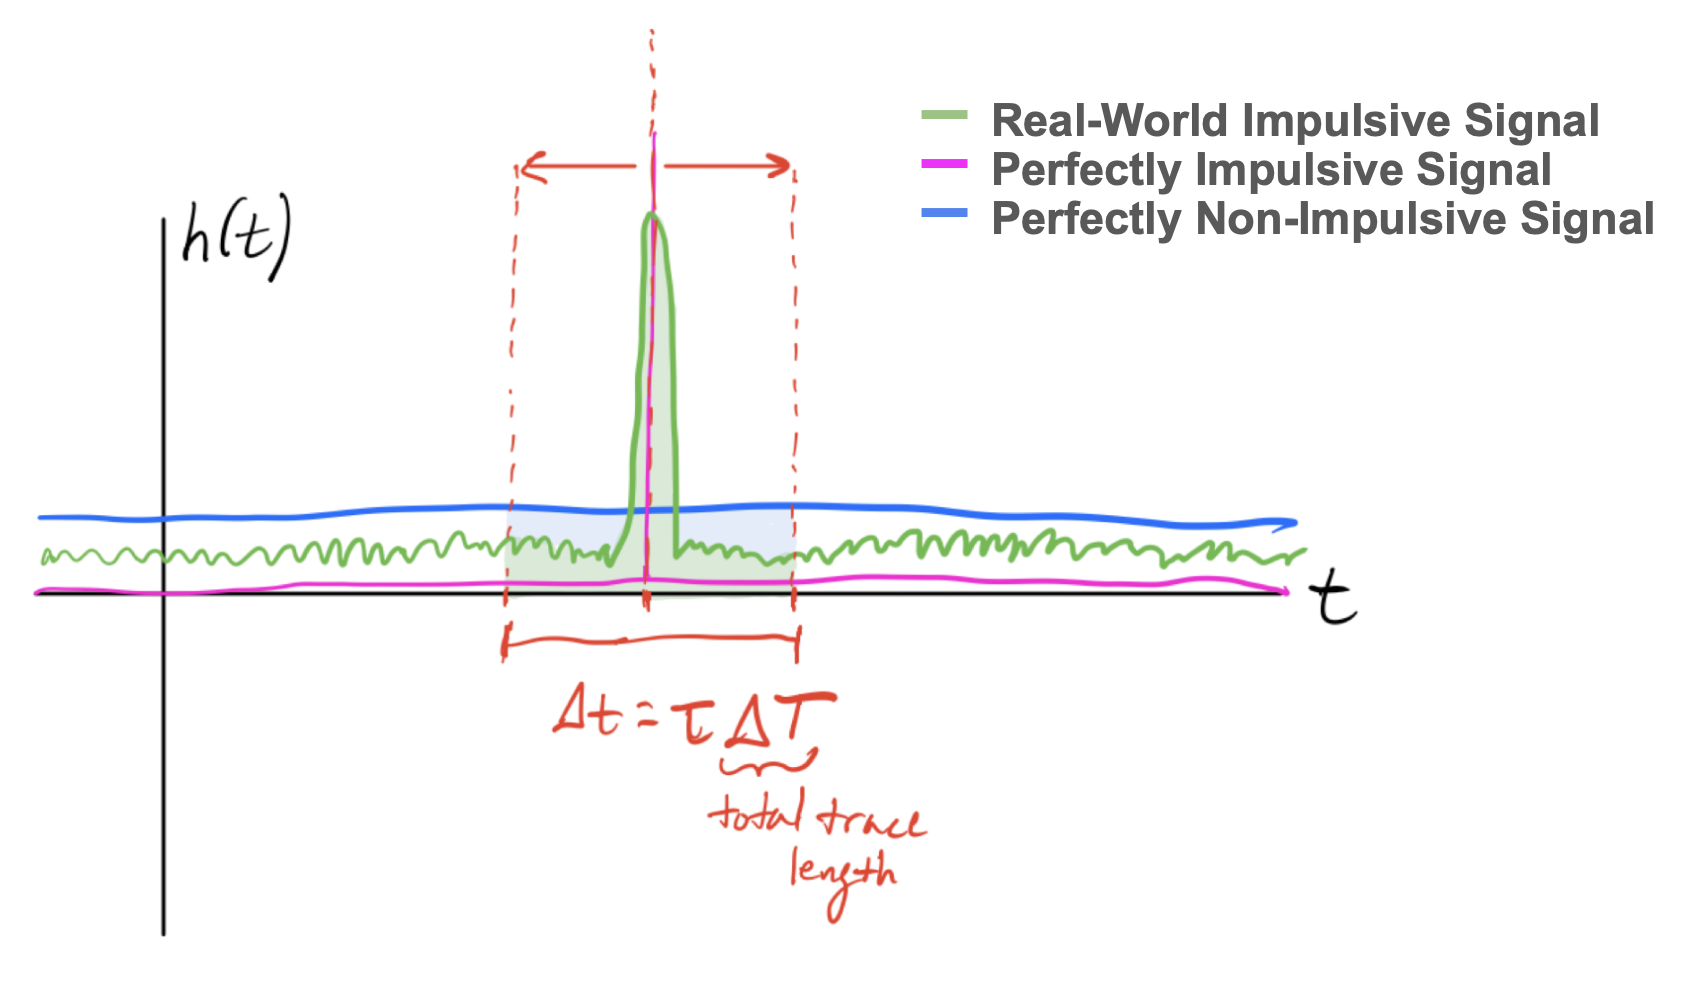
\includegraphics[width=\textwidth]{sections/5sa-cleaning/images_variables/impulsivity_waveforms.png}
      \end{subfigure}
      ~
      \begin{subfigure}[t]{0.48\textwidth}
        \centering
        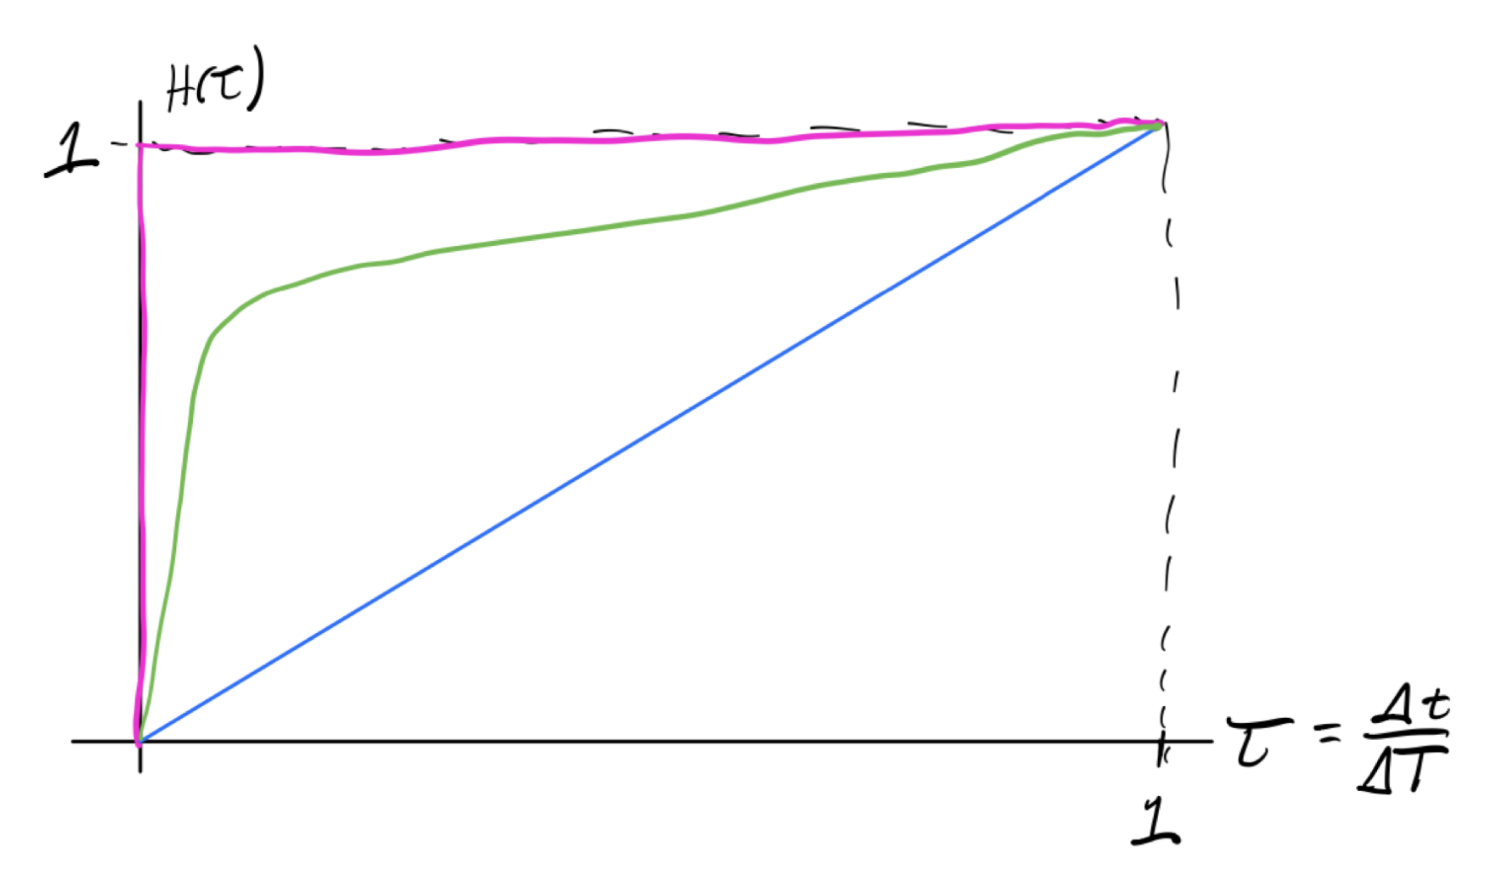
\includegraphics[width=\textwidth]{sections/5sa-cleaning/images_variables/impulsivity_cdfs.png}
      \end{subfigure}
      \caption{Left, cartoons of Hilbert enveloped waveforms for a real-world impulsive event (green), a perfectly impulsive event (pink), and a perfectly non-impulsive event. Right, cartoons of the corresponding impulsivity cumulative distribution function for each waveform shown on the left. }
      \label{fig:impulsivity_cdfs}
    \end{figure}

  \subsection{\texttt{impulsivity}}

      The impulsivity is calculated as 
      \begin{equation}
        \texttt{impulsivity} = \frac{1}{2} \overline{CDF} - 1
        \label{eq:impulsivity}
      \end{equation}
      where $\overline{CDF}$ is the average value of the impulsivity cumulative distribution function for this event's CSW.
      Example distributions are show in Figure~\ref{fig:impulsivity}.
    
      \begin{figure}
        \centering
        \begin{subfigure}[t]{0.48\textwidth}
          \centering
          \includegraphics[width=\textwidth]{sections/5sa-cleaning/images_variables/a2nu_1d_impulsivity_v.pdf}
        \end{subfigure}
        ~
        \begin{subfigure}[t]{0.48\textwidth}
          \centering
          \includegraphics[width=\textwidth]{sections/5sa-cleaning/images_variables/a2_10pct_1d_impulsivity_v.pdf}
        \end{subfigure}
        ~
        \begin{subfigure}[t]{0.48\textwidth}
          \centering
          \includegraphics[width=\textwidth]{sections/5sa-cleaning/images_variables/a2nu_2d_impulsivity_v_vs_avg_snr_v_rf.pdf}
        \end{subfigure}
        ~
        \begin{subfigure}[t]{0.48\textwidth}
          \centering
          \includegraphics[width=\textwidth]{sections/5sa-cleaning/images_variables/a2nu_2d_impulsivity_v_vs_global_max_corr_rf.pdf}
        \end{subfigure}
        \caption{
          Top, 1-dimensional distributions of simulated neutrinos following an $E^{-2}$ spectrum (top left) and data (top right) for the analysis variable \texttt{impulsivity\_v}. 
          The distribution of data has had all cuts applied to RF events except for the final thermal LDA cut described in Section~\ref{sec:lda}.
          The purple curve (which exactly overlays the orange curve) shows these RF events, blue shows software triggered events, and green shows calibration pulser events.
          Bottom, 2-dimensional distributions of simulated neutrinos for the analysis variable \texttt{impulsivity\_v} as a function of \texttt{avg\_snr\_v} and \texttt{global\_max\_corr\_v}.
        }
        \label{fig:impulsivity}
      \end{figure}

  \pagebreak
  \subsection{Linear Fit Parameters \label{sec:imp_linearfit}}

      One way to describe an event's impulsivity is to perform a linear fit to an event's impulsivity CDF. 
      \begin{equation}
        y = mx + b
        \label{eq:linear}
      \end{equation}
      Perfectly non-impulsive events should be well described by this fit, as shown in Figure~\ref{fig:impulsivity_cdfs}. 
      For impulsive events, the y-intercept roughly characterizes how much power is in a signal. 
      Examples of linear fits performed to real data are shown in Figure~\ref{fig:linearimp}.

    \begin{figure}[!ht]
      \centering
      \begin{subfigure}[t]{0.48\textwidth}
        \centering
        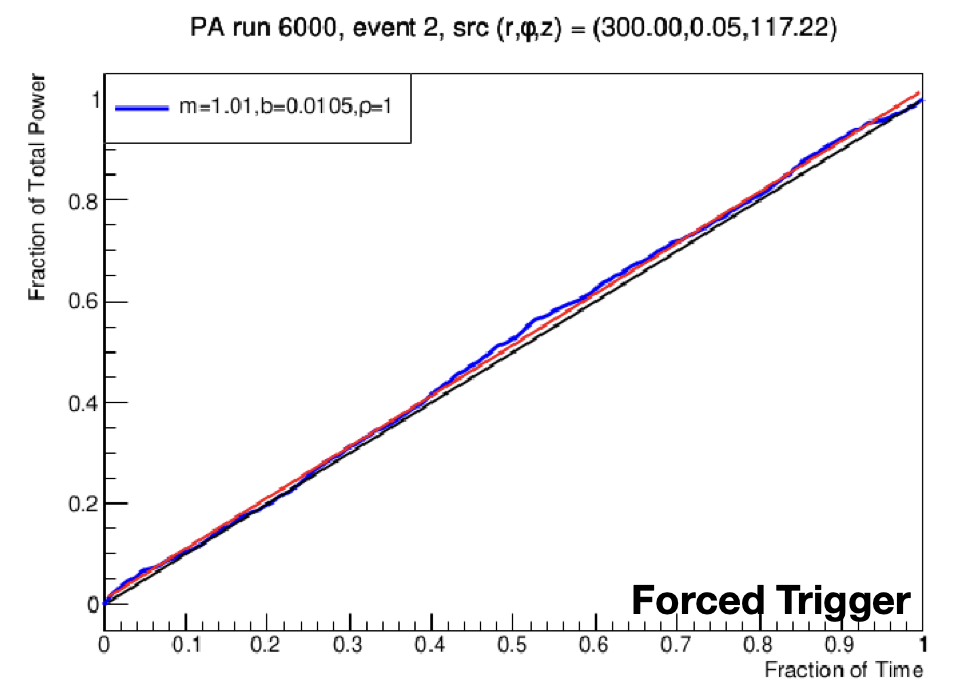
\includegraphics[width=\textwidth]{sections/5sa-analysis/plots/impLin_force_PA.png}
      \end{subfigure}
      ~
      \begin{subfigure}[t]{0.48\textwidth}
        \centering
        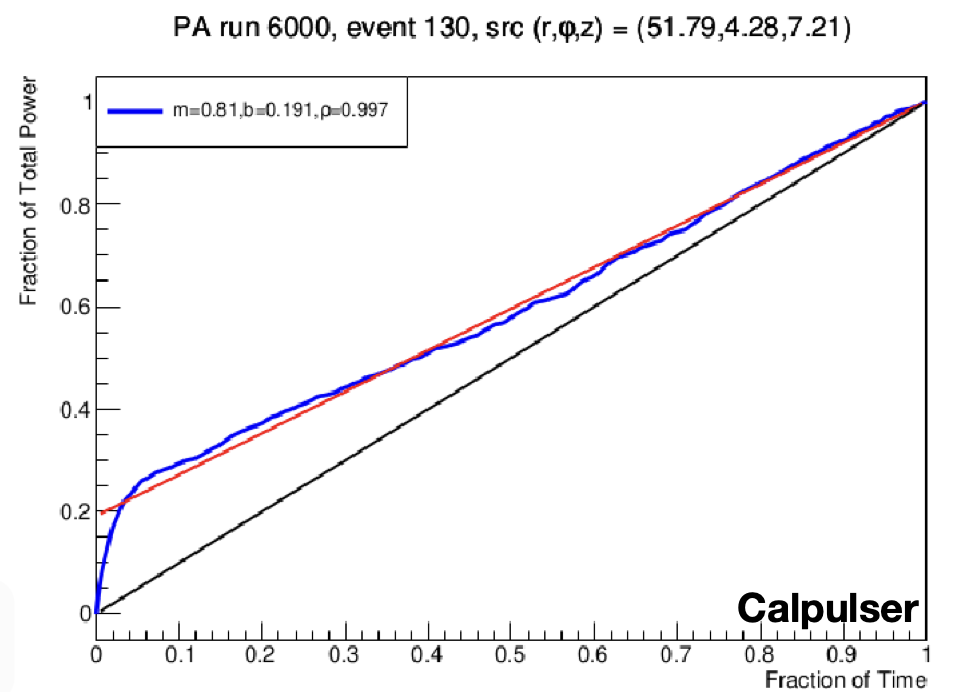
\includegraphics[width=\textwidth]{sections/5sa-analysis/plots/impLin_cp_PA.png}
      \end{subfigure}
      \caption{Example of a linear fit to an event's impulsivity curve courtesy of Marco Muzio.}
      \label{fig:linearimp}
    \end{figure}

    \subsubsection{\texttt{bImp}}

      This variable corresponds to the y-intercept of the linear fit calculated on a waveform's impulsivity CDF.
      Example distributions are shown in Figure~\ref{fig:bImp}.
    
      \begin{figure}
        \centering
        \begin{subfigure}[t]{0.48\textwidth}
          \centering
          \includegraphics[width=\textwidth]{sections/5sa-cleaning/images_variables/a2nu_1d_bImp_v.pdf}
        \end{subfigure}
        ~
        \begin{subfigure}[t]{0.48\textwidth}
          \centering
          \includegraphics[width=\textwidth]{sections/5sa-cleaning/images_variables/a2_10pct_1d_bImp_v.pdf}
        \end{subfigure}
        ~
        \begin{subfigure}[t]{0.48\textwidth}
          \centering
          \includegraphics[width=\textwidth]{sections/5sa-cleaning/images_variables/a2nu_2d_bImp_v_vs_avg_snr_v_rf.pdf}
        \end{subfigure}
        ~
        \begin{subfigure}[t]{0.48\textwidth}
          \centering
          \includegraphics[width=\textwidth]{sections/5sa-cleaning/images_variables/a2nu_2d_bImp_v_vs_global_max_corr_rf.pdf}
        \end{subfigure}
        \caption{
          Top, 1-dimensional distributions of simulated neutrinos following an $E^{-2}$ spectrum (top left) and data (top right) for the analysis variable \texttt{bImp\_v}. 
          The distribution of data has had all cuts applied to RF events except for the final thermal LDA cut described in Section~\ref{sec:lda}.
          The purple curve (which exactly overlays the orange curve) shows these RF events, blue shows software triggered events, and green shows calibration pulser events.
          Bottom, 2-dimensional distributions of simulated neutrinos for the analysis variable \texttt{bImp\_v} as a function of \texttt{avg\_snr\_v} and \texttt{global\_max\_corr\_v}.
        }
        \label{fig:bImp}
      \end{figure}
    
    \subsubsection{\texttt{mImp}}
    
      This variable corresponds to the slope of the linear fit calculated on a waveform's impulsivity CDF.
      Example distributions are shown in Figure~\ref{fig:mImp}.

      \begin{figure}
        \centering
        \begin{subfigure}[t]{0.48\textwidth}
          \centering
          \includegraphics[width=\textwidth]{sections/5sa-cleaning/images_variables/a2nu_1d_mImp_v.pdf}
        \end{subfigure}
        ~
        \begin{subfigure}[t]{0.48\textwidth}
          \centering
          \includegraphics[width=\textwidth]{sections/5sa-cleaning/images_variables/a2_10pct_1d_mImp_v.pdf}
        \end{subfigure}
        ~
        \begin{subfigure}[t]{0.48\textwidth}
          \centering
          \includegraphics[width=\textwidth]{sections/5sa-cleaning/images_variables/a2nu_2d_mImp_v_vs_avg_snr_v_rf.pdf}
        \end{subfigure}
        ~
        \begin{subfigure}[t]{0.48\textwidth}
          \centering
          \includegraphics[width=\textwidth]{sections/5sa-cleaning/images_variables/a2nu_2d_mImp_v_vs_global_max_corr_rf.pdf}
        \end{subfigure}
        \caption{
          Top, 1-dimensional distributions of simulated neutrinos following an $E^{-2}$ spectrum (top left) and data (top right) for the analysis variable \texttt{mImp\_v}. 
          The distribution of data has had all cuts applied to RF events except for the final thermal LDA cut described in Section~\ref{sec:lda}.
          The purple curve (which exactly overlays the orange curve) shows these RF events, blue shows software triggered events, and green shows calibration pulser events.
          Bottom, 2-dimensional distributions of simulated neutrinos for the analysis variable \texttt{mImp\_v} as a function of \texttt{avg\_snr\_v} and \texttt{global\_max\_corr\_v}.
        }
        \label{fig:mImp}
      \end{figure}
    
    \subsubsection{\texttt{rhoImp}}

      This variable corresponds to the correlation coefficient, $\rho$, of the linear fit calculated on a waveform's impulsivity CDF.
      Example distributions are shown in Figure~\ref{fig:rhoImp}.
    
      \begin{figure}
        \centering
        \begin{subfigure}[t]{0.48\textwidth}
          \centering
          \includegraphics[width=\textwidth]{sections/5sa-cleaning/images_variables/a2nu_1d_rhoImp_v.pdf}
        \end{subfigure}
        ~
        \begin{subfigure}[t]{0.48\textwidth}
          \centering
          \includegraphics[width=\textwidth]{sections/5sa-cleaning/images_variables/a2_10pct_1d_rhoImp_v.pdf}
        \end{subfigure}
        ~
        \begin{subfigure}[t]{0.48\textwidth}
          \centering
          \includegraphics[width=\textwidth]{sections/5sa-cleaning/images_variables/a2nu_2d_rhoImp_v_vs_avg_snr_v_rf.pdf}
        \end{subfigure}
        ~
        \begin{subfigure}[t]{0.48\textwidth}
          \centering
          \includegraphics[width=\textwidth]{sections/5sa-cleaning/images_variables/a2nu_2d_rhoImp_v_vs_global_max_corr_rf.pdf}
        \end{subfigure}
        \caption{
          Top, 1-dimensional distributions of simulated neutrinos following an $E^{-2}$ spectrum (top left) and data (top right) for the analysis variable \texttt{rhoImp\_v}. 
          The distribution of data has had all cuts applied to RF events except for the final thermal LDA cut described in Section~\ref{sec:lda}.
          The purple curve (which exactly overlays the orange curve) shows these RF events, blue shows software triggered events, and green shows calibration pulser events.
          Bottom, 2-dimensional distributions of simulated neutrinos for the analysis variable \texttt{rhoImp\_v} as a function of \texttt{avg\_snr\_v} and \texttt{global\_max\_corr\_v}.
        }
        \label{fig:rhoImp}
      \end{figure}

    \subsubsection{\texttt{impLinChi2}}

      This variable corresponds to the $\Chi^2$ calculated for a waveform's impulsivity CDF and its linear fit.
      Example distributions are shown in Figure~\ref{fig:impLinChi2}.
    
      \begin{figure}
        \centering
        \begin{subfigure}[t]{0.48\textwidth}
          \centering
          \includegraphics[width=\textwidth]{sections/5sa-cleaning/images_variables/a2nu_1d_impLinChi2_v.pdf}
        \end{subfigure}
        ~
        \begin{subfigure}[t]{0.48\textwidth}
          \centering
          \includegraphics[width=\textwidth]{sections/5sa-cleaning/images_variables/a2_10pct_1d_impLinChi2_v.pdf}
        \end{subfigure}
        ~
        \begin{subfigure}[t]{0.48\textwidth}
          \centering
          \includegraphics[width=\textwidth]{sections/5sa-cleaning/images_variables/a2nu_2d_impLinChi2_v_vs_avg_snr_v_rf.pdf}
        \end{subfigure}
        ~
        \begin{subfigure}[t]{0.48\textwidth}
          \centering
          \includegraphics[width=\textwidth]{sections/5sa-cleaning/images_variables/a2nu_2d_impLinChi2_v_vs_global_max_corr_rf.pdf}
        \end{subfigure}
        \caption{
          Top, 1-dimensional distributions of simulated neutrinos following an $E^{-2}$ spectrum (top left) and data (top right) for the analysis variable \texttt{impLinChi2\_v}. 
          The distribution of data has had all cuts applied to RF events except for the final thermal LDA cut described in Section~\ref{sec:lda}.
          The purple curve (which exactly overlays the orange curve) shows these RF events, blue shows software triggered events, and green shows calibration pulser events.
          Bottom, 2-dimensional distributions of simulated neutrinos for the analysis variable \texttt{impLinChi2\_v} as a function of \texttt{avg\_snr\_v} and \texttt{global\_max\_corr\_v}.
        }
        \label{fig:impLinChi2}
      \end{figure}


  \pagebreak
  \subsection{Functional Fit Parameters \label{sec:imp_functionalfit}}

    The functional fit uses an equation that roughly describes the Hilbert envelope of a real impulsive signal
    \begin{equation}
      h(t) \propto A e^{- t^2 / B^2 } + 1
      \label{eq:hilbert}
    \end{equation}
    to derive an equation describing the corresponding impulsivity CDF:
    \begin{equation}
      H(\tau) = \frac{ A ~ \text{erf}( \tau / B ) + \tau }{ A ~ \text{erf}( 1 / B ) + 1}
      \label{eq:functionalimp}
    \end{equation}
    where $A$ and $B$ are fit parameters, $\tau$ corresponds to the fraction of time in the waveform, and erf is the error response function. 
    An example of this functional fit applied to real data is shown in Figure~\ref{eq:functionalimp}.

    \begin{figure}[!ht]
      \centering
      \begin{subfigure}[t]{0.48\textwidth}
        \centering
        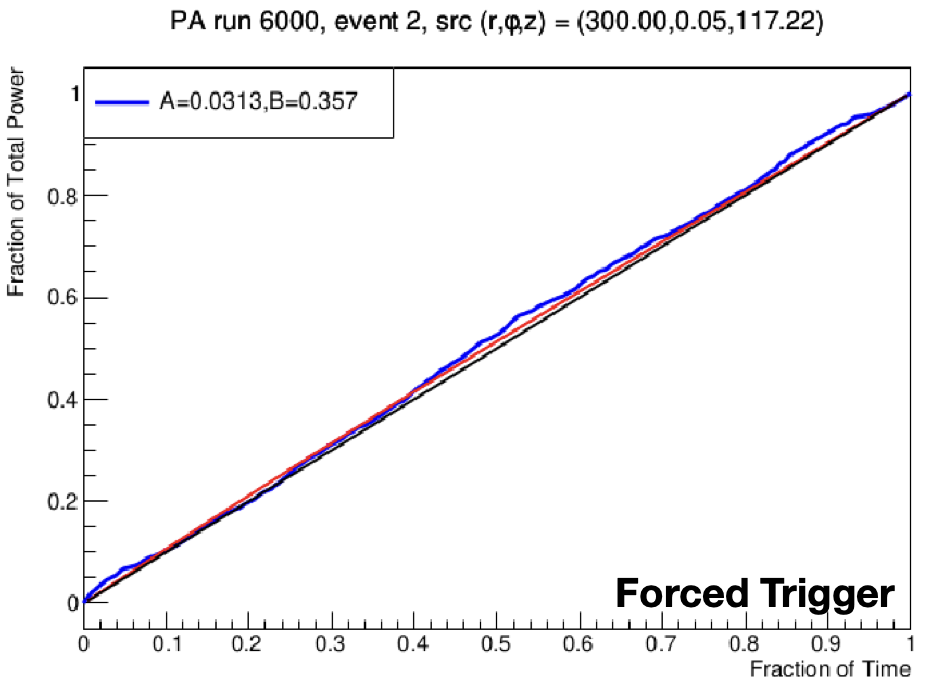
\includegraphics[width=\textwidth]{sections/5sa-analysis/plots/impErf_force_PA.png}
      \end{subfigure}
      ~
      \begin{subfigure}[t]{0.48\textwidth}
        \centering
        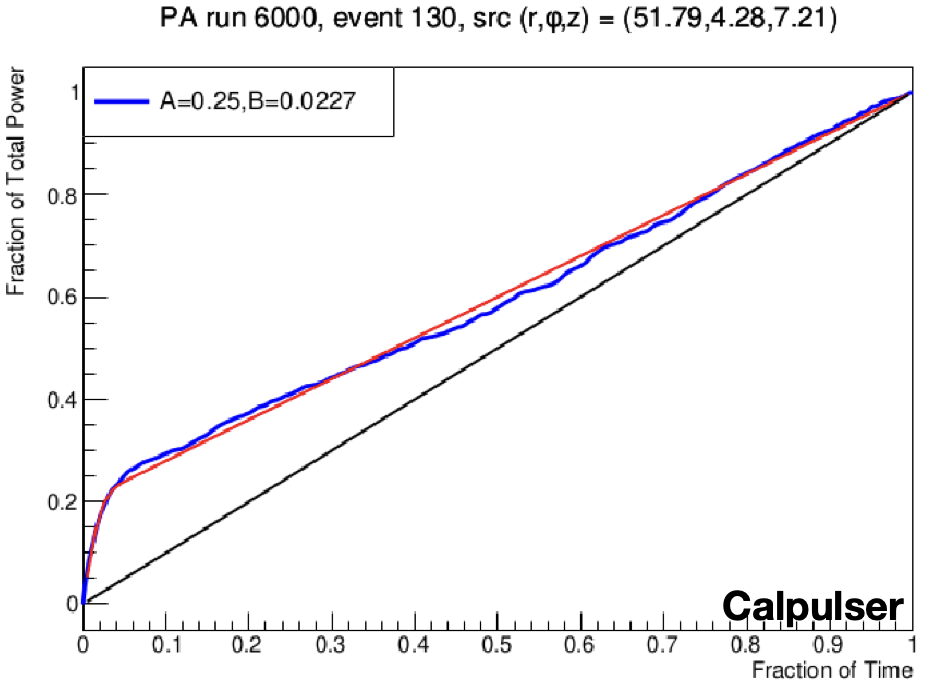
\includegraphics[width=\textwidth]{sections/5sa-analysis/plots/impErf_cp_PA.png}
      \end{subfigure}
      \caption{Example of the hilbert-inspired curve given by Equation~\ref{eq:functionalimp} fit to an event's impulsivity curve.}
      \label{fig:functionalimp}
    \end{figure}
    
    \subsubsection{\texttt{impErfA}}

      This variable corresponds to fit parameter $A$ of the functional impulsivity fit calculated on a waveform's impulsivity CDF, as defined in Equation~\ref{eq:functionalimp}.
      Example distributions are shown in Figure~\ref{fig:impErfA}.
    
      \begin{figure}
        \centering
        \begin{subfigure}[t]{0.48\textwidth}
          \centering
          \includegraphics[width=\textwidth]{sections/5sa-cleaning/images_variables/a2nu_1d_impErfA_v.pdf}
        \end{subfigure}
        ~
        \begin{subfigure}[t]{0.48\textwidth}
          \centering
          \includegraphics[width=\textwidth]{sections/5sa-cleaning/images_variables/a2_10pct_1d_impErfA_v.pdf}
        \end{subfigure}
        ~
        \begin{subfigure}[t]{0.48\textwidth}
          \centering
          \includegraphics[width=\textwidth]{sections/5sa-cleaning/images_variables/a2nu_2d_impErfA_v_vs_avg_snr_v_rf.pdf}
        \end{subfigure}
        ~
        \begin{subfigure}[t]{0.48\textwidth}
          \centering
          \includegraphics[width=\textwidth]{sections/5sa-cleaning/images_variables/a2nu_2d_impErfA_v_vs_global_max_corr_rf.pdf}
        \end{subfigure}
        \caption{
          Top, 1-dimensional distributions of simulated neutrinos following an $E^{-2}$ spectrum (top left) and data (top right) for the analysis variable \texttt{impErfA\_v}. 
          The distribution of data has had all cuts applied to RF events except for the final thermal LDA cut described in Section~\ref{sec:lda}.
          The purple curve (which exactly overlays the orange curve) shows these RF events, blue shows software triggered events, and green shows calibration pulser events.
          Bottom, 2-dimensional distributions of simulated neutrinos for the analysis variable \texttt{impErfA\_v} as a function of \texttt{avg\_snr\_v} and \texttt{global\_max\_corr\_v}.
        }
        \label{fig:impErfA}
      \end{figure}
    
    \subsubsection{\texttt{impErfB}}

      This variable corresponds to fit parameter $B$ of the functional impulsivity fit calculated on a waveform's impulsivity CDF, as defined in Equation~\ref{eq:functionalimp}.
      Example distributions are shown in Figure~\ref{fig:impErfB}.
    
      \begin{figure}
        \centering
        \begin{subfigure}[t]{0.48\textwidth}
          \centering
          \includegraphics[width=\textwidth]{sections/5sa-cleaning/images_variables/a2nu_1d_impErfB_v.pdf}
        \end{subfigure}
        ~
        \begin{subfigure}[t]{0.48\textwidth}
          \centering
          \includegraphics[width=\textwidth]{sections/5sa-cleaning/images_variables/a2_10pct_1d_impErfB_v.pdf}
        \end{subfigure}
        ~
        \begin{subfigure}[t]{0.48\textwidth}
          \centering
          \includegraphics[width=\textwidth]{sections/5sa-cleaning/images_variables/a2nu_2d_impErfB_v_vs_avg_snr_v_rf.pdf}
        \end{subfigure}
        ~
        \begin{subfigure}[t]{0.48\textwidth}
          \centering
          \includegraphics[width=\textwidth]{sections/5sa-cleaning/images_variables/a2nu_2d_impErfB_v_vs_global_max_corr_rf.pdf}
        \end{subfigure}
        \caption{
          Top, 1-dimensional distributions of simulated neutrinos following an $E^{-2}$ spectrum (top left) and data (top right) for the analysis variable \texttt{impErfB\_v}. 
          The distribution of data has had all cuts applied to RF events except for the final thermal LDA cut described in Section~\ref{sec:lda}.
          The purple curve (which exactly overlays the orange curve) shows these RF events, blue shows software triggered events, and green shows calibration pulser events.
          Bottom, 2-dimensional distributions of simulated neutrinos for the analysis variable \texttt{impErfB\_v} as a function of \texttt{avg\_snr\_v} and \texttt{global\_max\_corr\_v}.
        }
        \label{fig:impErfB}
      \end{figure}
    
    \subsubsection{\texttt{impErfLinChi2}}

      This variable corresponds to the $\Chi^2$ calculated for the functional impulsivity fit of a waveform's impulsivity CDF.
      Example distributions are shown in Figure~\ref{fig:impErfLinChi2}.
    
      \begin{figure}
        \centering
        \begin{subfigure}[t]{0.48\textwidth}
          \centering
          \includegraphics[width=\textwidth]{sections/5sa-cleaning/images_variables/a2nu_1d_impErfLinChi2_v.pdf}
        \end{subfigure}
        ~
        \begin{subfigure}[t]{0.48\textwidth}
          \centering
          \includegraphics[width=\textwidth]{sections/5sa-cleaning/images_variables/a2_10pct_1d_impErfLinChi2_v.pdf}
        \end{subfigure}
        ~
        \begin{subfigure}[t]{0.48\textwidth}
          \centering
          \includegraphics[width=\textwidth]{sections/5sa-cleaning/images_variables/a2nu_2d_impErfLinChi2_v_vs_avg_snr_v_rf.pdf}
        \end{subfigure}
        ~
        \begin{subfigure}[t]{0.48\textwidth}
          \centering
          \includegraphics[width=\textwidth]{sections/5sa-cleaning/images_variables/a2nu_2d_impErfLinChi2_v_vs_global_max_corr_rf.pdf}
        \end{subfigure}
        \caption{
          Top, 1-dimensional distributions of simulated neutrinos following an $E^{-2}$ spectrum (top left) and data (top right) for the analysis variable \texttt{impErfLinChi2\_v}. 
          The distribution of data has had all cuts applied to RF events except for the final thermal LDA cut described in Section~\ref{sec:lda}.
          The purple curve (which exactly overlays the orange curve) shows these RF events, blue shows software triggered events, and green shows calibration pulser events.
          Bottom, 2-dimensional distributions of simulated neutrinos for the analysis variable \texttt{impErfLinChi2\_v} as a function of \texttt{avg\_snr\_v} and \texttt{global\_max\_corr\_v}.
        }
        \label{fig:impErfLinChi2}
      \end{figure}
    
  \subsection{\texttt{impSig}}

      This variable calculates the significance of the functional fit (defined in Section~\ref{sec:imp_functionalfit}) compared to the linear fit (defined in Section~\ref{sec:imp_linearfit}).
      Example distributions are shown in Figure~\ref{fig:impSig}.
    
      \begin{figure}
        \centering
        \begin{subfigure}[t]{0.48\textwidth}
          \centering
          \includegraphics[width=\textwidth]{sections/5sa-cleaning/images_variables/a2nu_1d_impSig_v.pdf}
        \end{subfigure}
        ~
        \begin{subfigure}[t]{0.48\textwidth}
          \centering
          \includegraphics[width=\textwidth]{sections/5sa-cleaning/images_variables/a2_10pct_1d_impSig_v.pdf}
        \end{subfigure}
        ~
        \begin{subfigure}[t]{0.48\textwidth}
          \centering
          \includegraphics[width=\textwidth]{sections/5sa-cleaning/images_variables/a2nu_2d_impSig_v_vs_avg_snr_v_rf.pdf}
        \end{subfigure}
        ~
        \begin{subfigure}[t]{0.48\textwidth}
          \centering
          \includegraphics[width=\textwidth]{sections/5sa-cleaning/images_variables/a2nu_2d_impSig_v_vs_global_max_corr_rf.pdf}
        \end{subfigure}
        \caption{
          Top, 1-dimensional distributions of simulated neutrinos following an $E^{-2}$ spectrum (top left) and data (top right) for the analysis variable \texttt{impSig\_v}. 
          The distribution of data has had all cuts applied to RF events except for the final thermal LDA cut described in Section~\ref{sec:lda}.
          The purple curve (which exactly overlays the orange curve) shows these RF events, blue shows software triggered events, and green shows calibration pulser events.
          Bottom, 2-dimensional distributions of simulated neutrinos for the analysis variable \texttt{impSig\_v} as a function of \texttt{avg\_snr\_v} and \texttt{global\_max\_corr\_v}.
        }
        \label{fig:impSig}
      \end{figure}

  % https://aradocs.wipac.wisc.edu/cgi-bin/DocDB/ShowDocument?docid=2964 impulsivity metrics
  
\pagebreak
\section{\texttt{mindepth\_v} \label{sec:mindepth}}

  \begin{figure}[!ht]
    \centering
    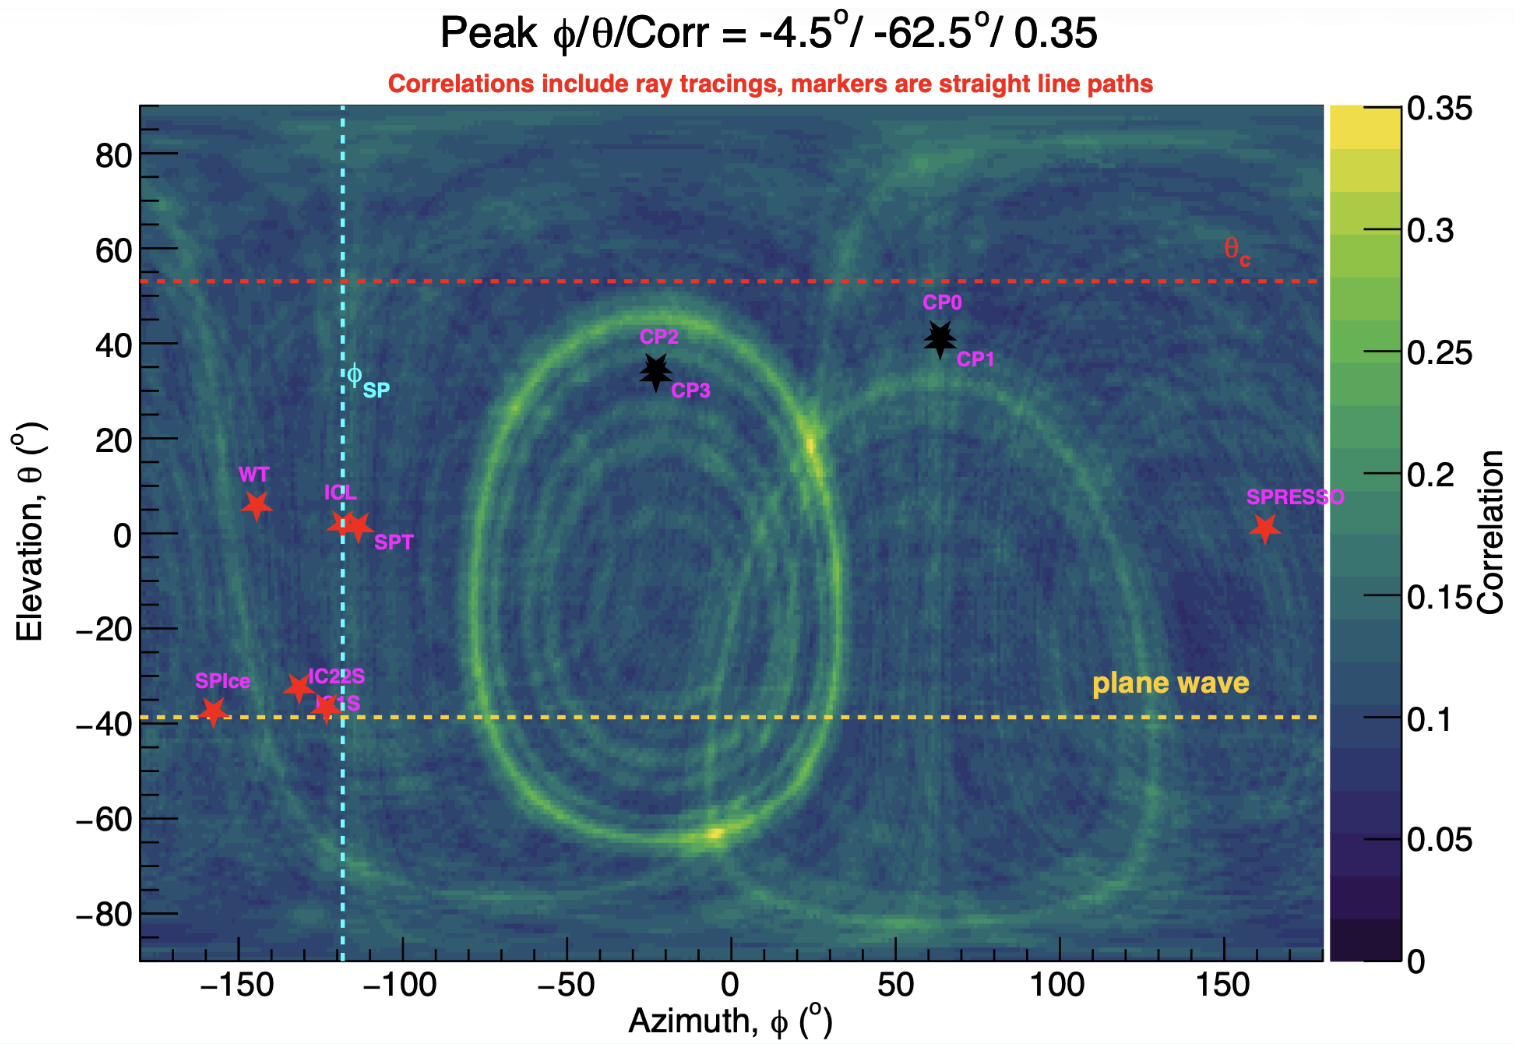
\includegraphics[
        width=0.75\textwidth,
        alt={}
    ]{sections/5sa-cleaning/images/a1r3183e65990_mindepth.pdf}
    \caption{An example of an event with a high \texttt{mindepth\_v}, meaning this event has many possible reconstructions that imply this event originated near the surface. This example is A1, run 3183, event 65990.}
    \label{fig:lowmindepth}
  \end{figure}

  This variable is calculated using the map of correlation values for all locations on the sky in azimuth and elevation to identify the highest elevation in the reconstruction map with a correlation value $\geq 60$\% of the map's maximimum correlation value.
  Taking Figure~\ref{fig:lowmindepth} for example, the maximum correlation value of this reconstruction skymap is 0.35 and we find the highest elevation a location on the sky with a correlation score of 0.21 ($0.6 \times 3.5$) is at an elevation of 68.5$^{\circ}$.
  We take this one step further and convert this maximum elevation angle into a minimum depth from the surface 
  \begin{equation}
    d = z_{\text{SC}} - r \sin{\theta}
    \label{eq:mindepth}
  \end{equation}
  where $z_{\text{SC}}$ is the average antenna depth for the station, $r$ is the radius of the reconstruction sphere, and $\theta$ is the elevation angle.
  For Figure~\ref{fig:lowmindepth}, which is the reconstruction of an A1 event using the pulser map radius (defined in Tab.~\ref{tab:cpdist}), $z_{\text{SC}}=-67.5$~m and $r=48.02$~m.
  This yields a \texttt{mindepth\_v}$=22.7$~m for this event. 
  This conversion to \texttt{mindepth\_v} was done to more easily compare our event reconstructions to the average depth of cosmic ray cores that impact into the ice - the deepest surface-related background we expect to observe, in theory.
  Example distributions are shown in Figure~\ref{fig:mindepthv}.
    
  \begin{figure}
    \centering
    \begin{subfigure}[t]{0.48\textwidth}
      \centering
      \includegraphics[width=\textwidth]{sections/5sa-cleaning/images_variables/a2nu_1d_mindepth_v.pdf}
    \end{subfigure}
    ~
    \begin{subfigure}[t]{0.48\textwidth}
      \centering
      \includegraphics[width=\textwidth]{sections/5sa-cleaning/images_variables/a2_10pct_1d_mindepth_v.pdf}
    \end{subfigure}
    ~
    \begin{subfigure}[t]{0.48\textwidth}
      \centering
      \includegraphics[width=\textwidth]{sections/5sa-cleaning/images_variables/a2nu_2d_mindepth_v_vs_avg_snr_v_rf.pdf}
    \end{subfigure}
    ~
    \begin{subfigure}[t]{0.48\textwidth}
      \centering
      \includegraphics[width=\textwidth]{sections/5sa-cleaning/images_variables/a2nu_2d_mindepth_v_vs_global_max_corr_rf.pdf}
    \end{subfigure}
    \caption{
      Top, 1-dimensional distributions of simulated neutrinos following an $E^{-2}$ spectrum (top left) and data (top right) for the analysis variable \texttt{mindepth\_v}. 
      The distribution of data has had all cuts applied to RF events except for the final thermal LDA cut described in Section~\ref{sec:lda}.
      The purple curve (which exactly overlays the orange curve) shows these RF events, blue shows software triggered events, and green shows calibration pulser events.
      Bottom, 2-dimensional distributions of simulated neutrinos for the analysis variable \texttt{mindepth\_v} as a function of \texttt{avg\_snr\_v} and \texttt{global\_max\_corr\_v}.
    }
    \label{fig:mindepthv}
  \end{figure}


\pagebreak
\section{\texttt{wavefront\_rms\_v}}

  \texttt{wavefront\_rms} is a measure of how compatible observed waveforms are with an arriving plane wave. 
  We use a simplified version of what was originally proposed by Carl Pfender and explained in~\citep{thesis_clark}
  For like-polarization antennas, we determine the time of maximum peak-to-peak (maximum-to-minimum) voltage in any 20 nanosecond window over the whole waveform.
  We then assume, for the purpose of this calculation, that the signal from a potential plane wave arrived at this antenna at this time of maximum peak-to-peak voltage separation.
  For each pair of antennas, the time difference between these maximum peak-to-peak times is used to calculate the arrival angle of the signal as
  \begin{equation}
    cos(\theta) = \frac{c \Delta t}{n \Delta d}
    \label{eq:wavefrontrms}
  \end{equation}
  where $c$ is the speed of light in a vacuum, $\Delta t$ is the time delay between antennas, $n$ is the refractive index of the medium (ice), and $\Delta d$ is the distance between the two antennas. 
  When comparing the arrival angle calculated by each pair of antennas, if a plane wave was observed then these arrival angles should all be similar. 
  If a thermal-like event was observed, then these calculated arrival angles should all be quite different from each other. 
  To quantify this, we calculate the variance of all the calculated arrival angles (contrary to the variable name of ``RMS'').
  When this variance, the \texttt{wavefront\_rms}, is small, the recorded waveform has a strong likelihood of originating from a plane wave and when it is large, this scenario is less likely.
  Example distributions are shown in Figure~\ref{fig:wavefront_rms}.
    
  \begin{figure}
    \centering
    \begin{subfigure}[t]{0.48\textwidth}
      \centering
      \includegraphics[width=\textwidth]{sections/5sa-cleaning/images_variables/a2nu_1d_wavefront_rms_v.pdf}
    \end{subfigure}
    ~
    \begin{subfigure}[t]{0.48\textwidth}
      \centering
      \includegraphics[width=\textwidth]{sections/5sa-cleaning/images_variables/a2_10pct_1d_wavefront_rms_v.pdf}
    \end{subfigure}
    ~
    \begin{subfigure}[t]{0.48\textwidth}
      \centering
      \includegraphics[width=\textwidth]{sections/5sa-cleaning/images_variables/a2nu_2d_wavefront_rms_v_vs_avg_snr_v_rf.pdf}
    \end{subfigure}
    ~
    \begin{subfigure}[t]{0.48\textwidth}
      \centering
      \includegraphics[width=\textwidth]{sections/5sa-cleaning/images_variables/a2nu_2d_wavefront_rms_v_vs_global_max_corr_rf.pdf}
    \end{subfigure}
    \caption{
      Top, 1-dimensional distributions of simulated neutrinos following an $E^{-2}$ spectrum (top left) and data (top right) for the analysis variable \texttt{wavefront\_rms\_v}. 
      The distribution of data has had all cuts applied to RF events except for the final thermal LDA cut described in Section~\ref{sec:lda}.
      The purple curve (which exactly overlays the orange curve) shows these RF events, blue shows software triggered events, and green shows calibration pulser events.
      Bottom, 2-dimensional distributions of simulated neutrinos for the analysis variable \texttt{wavefront\_rms\_v} as a function of \texttt{avg\_snr\_v} and \texttt{global\_max\_corr\_v}.
    }
    \label{fig:wavefront_rms}
  \end{figure}

